\documentclass[a4paper,11pt]{article}
\usepackage[big]{layaureo}
\usepackage{amsmath,amssymb}
\usepackage[regular,semibold]{sourceserifpro}
\usepackage[regular,semibold]{sourcesanspro}
\usepackage[T1]{fontenc}
\usepackage[utf8]{inputenc}
\usepackage{textcomp} % provide euro and other symbols
\usepackage[]{microtype}
\usepackage{xcolor}
\usepackage{longtable,booktabs,array}
\usepackage{calc} % for calculating minipage widths
\usepackage{pdfpages}
\usepackage{graphicx}
\usepackage{sectsty}
\usepackage{setspace}
\usepackage[hidelinks]{hyperref}
\usepackage{hyperxmp}
\usepackage[
    type={CC},
    modifier={zero},
    version={1.0},
]{doclicense}
\usepackage{outlines}
\usepackage{enumitem}
\usepackage{subcaption}
\usepackage{svg}
\usepackage{wrapfig}

\def\documenttitle{Cash or Card?}
\def\documentauthor{Andrea Franceschini}
\def\documentsubject{Game Design Document}
\def\documentversion{1.1}
\def\documentdate{2023-10-13}
\def\documentcreationdate{2023-07-01}

\hypersetup{
pdftitle={\documenttitle},
pdfauthor={\documentauthor},
pdfcreationdate={\documentcreationdate},
pdfmoddate={\documentdate},
pdfmetadate={\documentdate},
pdfversionid={\documentversion},
pdflang={en-GB},
pdfsubject={{\documentsubject}},
}

\title{\documenttitle}
\author{\documentauthor}

\onehalfspacing

\makeatletter
\renewcommand{\maketitle}{\bgroup\setlength{\parindent}{0pt}
\begin{flushleft}
	\sffamily\LARGE\@title
\end{flushleft}\egroup
}
\makeatother

\begin{document}

\maketitle\vspace{\baselineskip}

\begin{table}[h!]
  \begin{tabular}{@{}ll}
  WP 2 (Scientific)   &                                                      \\
  Version             & \documentversion                                     \\
  Creation Date       & \documentdate                                        \\
  Document Type    & Game Design Document                                 \\
  Dissemination level & Public                                               \\
  Author              & \documentauthor\ (\href{mailto:andrea.franceschini.2@unipd.it}{andrea.franceschini.2@unipd.it})
  \end{tabular}
\end{table}

\begin{wrapfigure}{l}{0pt}
  \raisebox{0pt}[\dimexpr\height-1.0\baselineskip\relax]{
\includegraphics[height=2\baselineskip]{figures/eu_flag.pdf}}
\end{wrapfigure}

\noindent Funded by the European Union\\ HORIZON-MSCA-2021-PF-01, Project ID 101062788 (EduGames)

\doclicenseThis
\vspace{2\baselineskip}

\noindent Help a shopkeeper get paid: customers prefer paying cash or card and you will decide whether to accept it or propose an alternative! Accept cash to feel it rustle between your fingers or embrace the convenience of electronic payments? The choice is yours! But be careful because every choice has consequences. Insurance premium or banking fees? Risk of robbery or losing a customer? Choose your strategy, see the consequences and explore the advantages, disadvantages and reasons behind each choice!

\vspace{\baselineskip}\noindent\textbf{Genre}: Puzzle, simulation

\vspace{\baselineskip}\noindent Developed as part of the EduGames project\\See \url{https://edugames.andreafranceschini.org} for more information.

\section{High level concept}\label{high-level-concept}
\subsection{Background and game experience}\label{background}
This game is about \textbf{the costs, risks, and opportunities of using cash and electronic payments in everyday purchases}. This is a hotly debated and complex theme, and there are no right or wrong answers. The game reflects this complexity by aiming for a presentation that is as neutral as possible, giving the player \textbf{freedom to adopt different strategies and explore their consequences}.

Being developed within the EduGames project, ``Cash or Card?'' is an educational game with entertainment ambitions. The EduGames project aims to develop design, development, and research guidelines for the creation and evaluation of video games that intend to educate through entertainment. Too often, educational video games have the reputation of being \emph{boring} and \emph{badly designed}. This is in contrast to most entertainment video games which captivate players for many hours and multiple play sessions. Continual and repeated engagement is desirable in education as it promotes deeper and repeated exploration of, and exposure to, the educational content. More information is provided in the project's website.

\subsection{Target audience}\label{target-audience}
General population.

\begin{itemize}
  \item Adults (18+) are the primary target audience as they are more likely to regularly handle payments and have a payment card or other electronic payment method.
  \item Young adults (13-18) are somewhat likely to handle payments, although they are unlikely to use non-cash payment methods. Young adults are an important target audience as they are soon going to turn into the primary audience, therefore it is important that they get early exposure to the content.
  \item Children (8-13) are a secondary target audience, although important in the long run, and because they can influence their parents and guardians. In financial matters, children tend to get exposed second-hand to choices made by their parents and guardians, and often take these choices acritically. It is important for them to be exposed to the different sides of the debate so that they can feel confident in asking questions and discussing it with adults.
\end{itemize}

\subsection{Unique selling points}\label{unique-selling-points}
In reality, there are more customers than shopkeepers. The shopkeepers tend to have very strong views and a very defensive attitude towards their preferred payment choices. It is not easy for customers to understand and discuss the shopkeepers' perspective -- i.e., \textit{trust me, you don't know what it's like to run a shop!} -- and so playing the role can be informative for customers.

\section{Product design}\label{product-design}
\subsection{Player experience and game POV}\label{player-experience-and-game-pov}
The player is a shopkeeper who must earn enough money to pay a big invoice within the next 5 days.

\subsection{Visual and Audio style}\label{visual-and-audio-style}
\begin{description}
  \item[Visuals:] retro-style pixel art visuals. The main play stage uses as background a cavalier view of the shop floor with a stylized representation of the shopkeeper and the customers. In the foreground, the player sees information about the current customer, the current state of the play, and the dialogue.
  \item[Audio:] chiptune-adjacent music and SFX. Background music plays during the ``day'' as background music in the shop. SFX are used to represent extraordinary events -- e.g., a shop robbery.
\end{description}

\subsection{Game World}\label{game-world}
The game is played entirely inside the shopkeeper's shop, with narrative implying events happening outside, i.e., bank runs, street robberies. The game opens with a phone call from one of the shopkeeper's suppliers reminding the shopkeeper they need to pay a big invoice by the end of the week. The shopkeeper states they have still 5 days to earn the remaining money. The game loop starts from there until the end of the game.

\subsection{Technology}\label{technology}
\subsubsection{Requirements}\label{technology-requirements}
The EduGames project requires that the games developed are open source, easy to maintain, and easy to access for players. This ensures that they remain playable and maintainable for as long as possible after the end of the project.

\subsubsection{Platforms}
The game will be playable on desktop computers and mobile phones. For maximum initial ease of deployment, the game will be published online as a Wasm\footnote{WebAssembly is a technology to deploy executables on the web and run them in the browser.} executable and accessible through browsers.

\subsubsection{Engine}
Godot 4 is the engine chosen because it satisfies the requirements gathered above. Godot 4 is open source, well documented, easy for beginners to learn and use, it is quickly becoming a favourite in the indie game development community, and it is making its way into the mainstream of commercial video games.\footnote{\url{https://godotengine.org/showcase/}} These characteristics guarantee maintainability for the foreseeable future.

\section{Detailed and Game Systems Design}\label{detailed-and-game-systems-design}
\subsection{Mechanics}\label{mechanics}
\subsubsection{Core loop}\label{core-loop}
The game loop runs 5 times (days) as follows. Every day is preceded by a day card summarising the current state of play.

\begin{enumerate}[label={\arabic{enumi}}]
\item \label{start} A customer (NPC, see \S\ref{customers}) approaches the check-out desk with an amount to pay and a payment preference (cash or card).
\item The player decides whether to take the payment offer or propose an alternative method.
\item \label{player-accepts} If the player accepts:

  \begin{enumerate}[label={\arabic{enumi}.\arabic{enumii}}]
  \item If the customer prefers card, the player is presented with three choices or payment methods with different payment fees. The fee is deducted from the total. The bank and electronic costs amounts are updated accordingly. Skip to step \ref{next}.
  \item If the customer prefers cash, the full amount is added to the cash amount. Skip to step \ref{next}.
  \end{enumerate}
\item If the player rejects:

  \begin{enumerate}[label={\arabic{enumi}.\arabic{enumii}}]
  \item A dialogue starts between the customer and the player with each party presenting a series of common objections to using the other payment method.
  \item The player can at any point give in to the customer's request, or insist in the hope of changing the customer's mind.
  \item If the customer leaves the goods and exits the shop without paying, the full amount is recorded as lost income. Skip to step \ref{next}
  \item If the customer or the player decide to accept a payment method, the payment is handled like in step \ref{player-accepts} using the payment method agreed so far.
  \end{enumerate}
\item \label{next} If there are still customers, the loop starts back from step \ref{start}.
\item If there are no more customers, the end of day scenario plays out.

  \begin{enumerate}[label={\arabic{enumi}.\arabic{enumii}}]
  \item If there is cash in the till, the player must decide whether to leave it there until the next day (back to step \ref{start}), or take it to the bank.
  \item \label{bank-run} If the player does a bank run, unless they run into a street robbery, a cash deposit fee is deducted from the cash amount and is added to the cash costs, and the remaining amount is added to the bank total. This represents that cash is not as \emph{gratis} as it may appear. The loop starts back from step \ref{start}.
  \item \label{street-robbery} If the player runs into a street robbery, based on the robbery chance, they have a choice of losing all the cash or making an insurance claim. If they make an insurance claim, they are refunded the cash amount minus the excess and the cash deposit fee, and the bank and cash costs are updated as in step \ref{bank-run}. The insurance premium and excess increase. The loop starts back from step \ref{start}.
  \end{enumerate}
\end{enumerate}

\subsubsection{Robbery risk}
At any point during a game loop (day) a shop robbery can happen based on the robbery chance. A shop robbery is handled like in step \ref{street-robbery} with the additional cost of losing any remaining customers for the day. The chance of robbery is calculated based on the amount of cash in possession of the player. There is a minimum probability of 0.5\%.

\subsubsection{End of game}
\textbf{Win condition:} after 5 loops (days), the total present in the bank minus the insurance premium is checked to see if there is enough available to pay the invoice.

Feedback is offered to the player as to the state of play. To be determined how to offer more tailored feedback based on how the player played the game.

\subsubsection{Customers}\label{customers}

Customers have a number of characteristics that determine their appearance and behaviour.
\begin{description}
  \item[Name:] chosen among the 100 most common given names in Italy, half males, half females.
  \item[Picture:] each name has a unique picture.
  \item[Cash preference:] random, 0-3. Determines how resolved the customer is to use cash. Decreased by 1 every time the player proposes to pay by card.
  \item[Must use cash:] random, true or false. A small percentage of customers (5\%) will use nothing but cash. This influences some of their dialogue choices to be more extreme and taking from various conspiracy theory thinking. If this is true, the cash preference is also set to an impossibly high value to avoid unintended edge cases.
  \item[Denial tolerance:] random, 2-4. Determines how many times a customer can take a counter-offer from the player. Decreased by 1 every time the player proposes another payment type. If it reaches zero, the customer either leaves the goods and does not pay, or accepts the alternate payment method.
  \item[Payment method:] based on cash preference, cash or card. This is the initial payment method proposed by the customer.
\end{description}

Customers are presented on screen with a somewhat vague verbal description of their cash preferences and denial tolerance. The player can use this to guess a strategy for each customer.

\subsection{Objectives and Progression}\label{objectives-and-progression}
The player's objective is to earn enough money at the end of 5 days to pay a large invoice plus the insurance premium. The player's actions are guided by the dialogues presented during the game loop.

\subsection{Game Systems}\label{game-systems}
In the first instance, the basic game system is entirely described by the core loop. There is scope for power-ups and side-mechanics to make the game more flexible and increase the player's control, freedom, and immersion.

\subsection{Wireframes and Interactivity}\label{interactivity}
Figure \ref{fig:screens} presents a selection of screens from the game. The main interaction system is the dialogue system shown in vignette (\subref{fig:gameplay}). Screens not presented in figure \ref{fig:screens} include
\begin{description}
  \item[Privacy:] a screen that informs the player about the type of anonymous data collection performed during the game.
  \item[Credits:] information about the artwork (visuals, music) and the technology used, and further information on the EduGames project.
\end{description}

\begin{figure}[p]
  \centering
  \begin{subfigure}{0.475\textwidth}
    \centering
    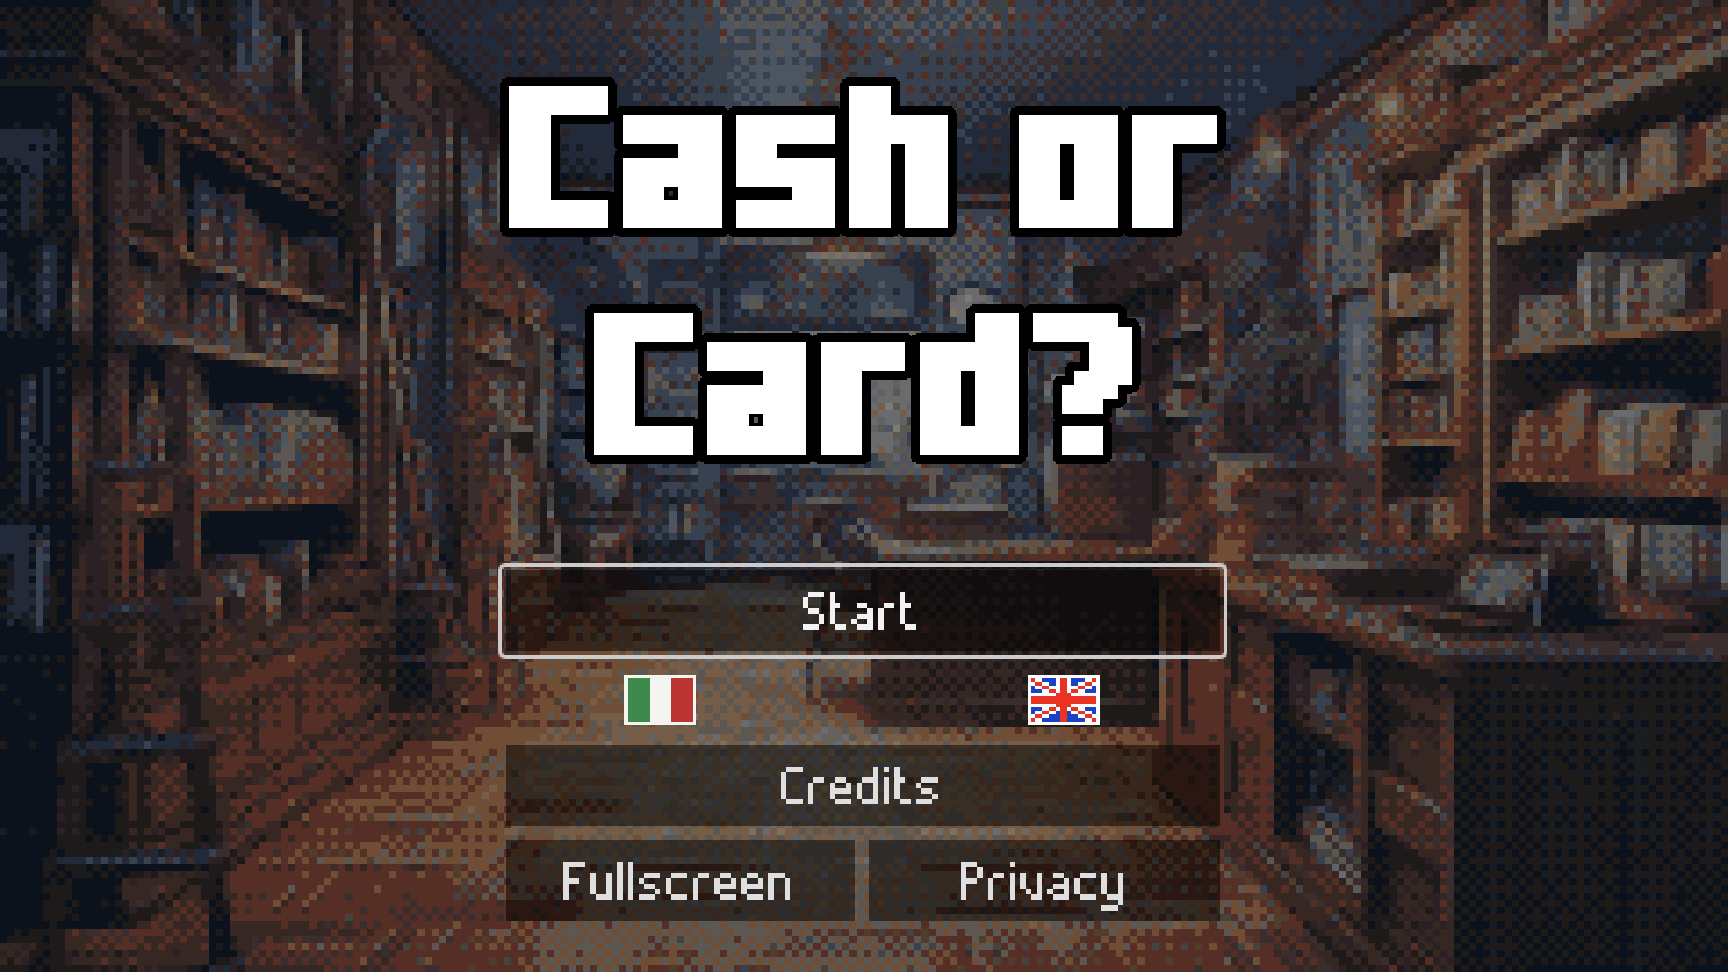
\includegraphics[width=\textwidth]{figures/title.png}
    \caption{Title screen}\label{fig:title}
  \end{subfigure}
  \hfill
  \begin{subfigure}{0.475\textwidth}
    \centering
    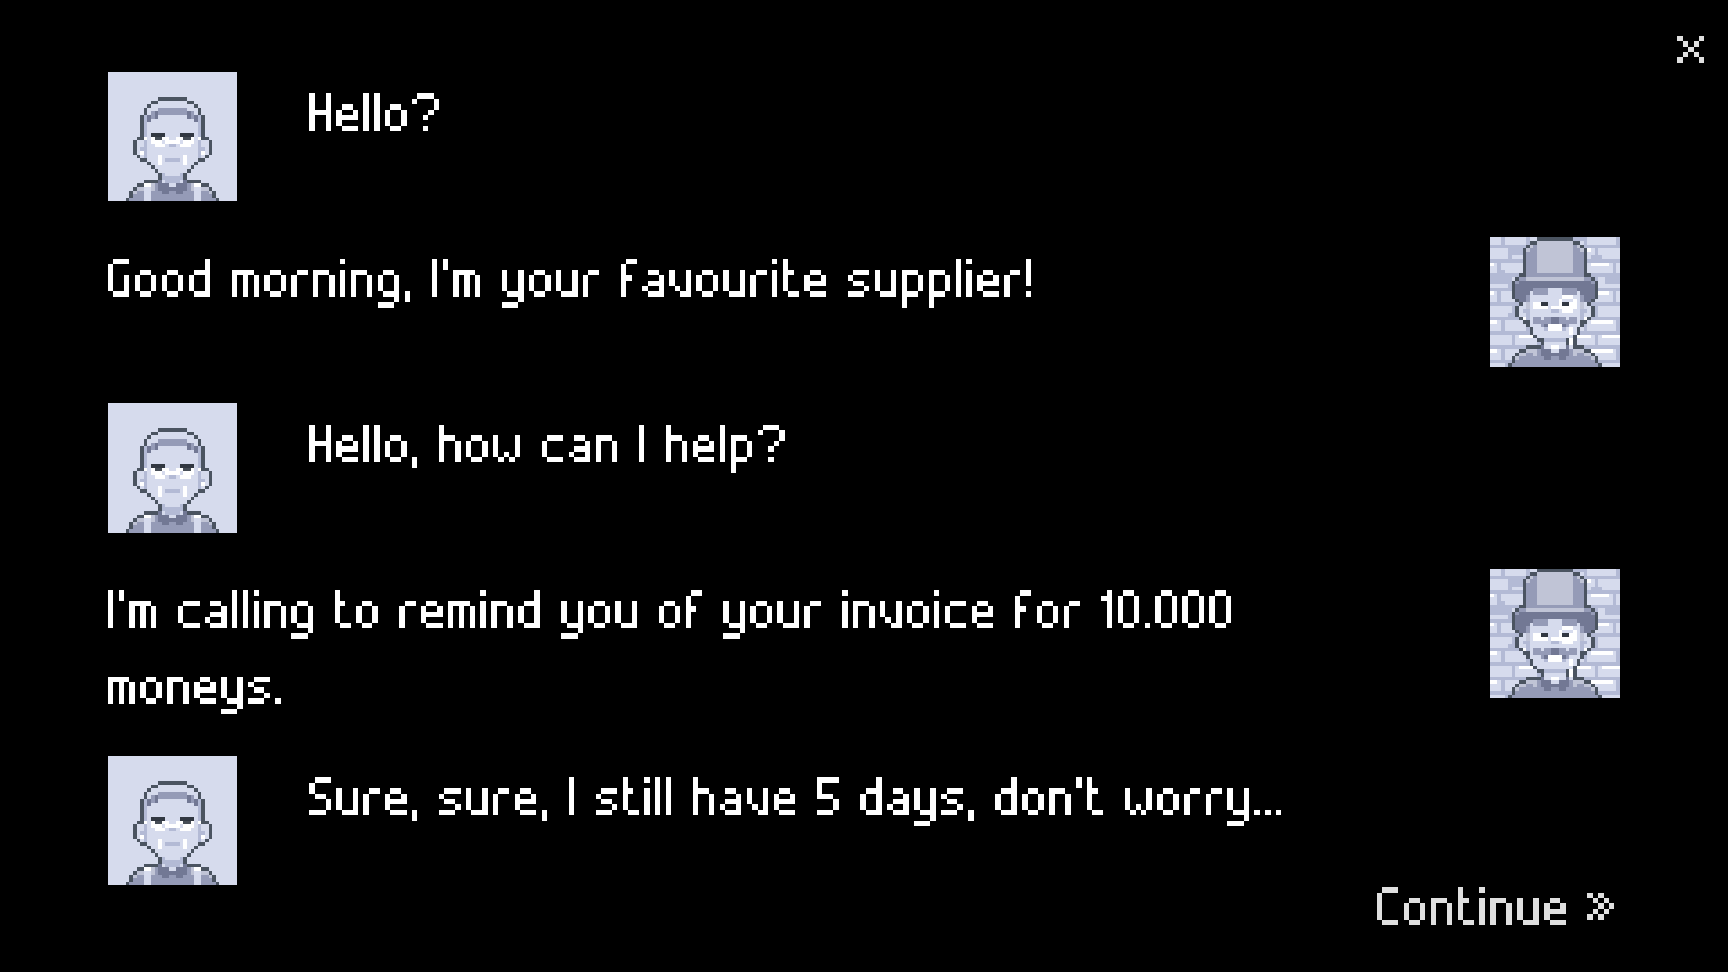
\includegraphics[width=\textwidth]{figures/story.png}
    \caption{Story introduction}\label{fig:story}
  \end{subfigure}

  \vspace{\baselineskip}
  \begin{subfigure}{0.475\textwidth}
    \centering
    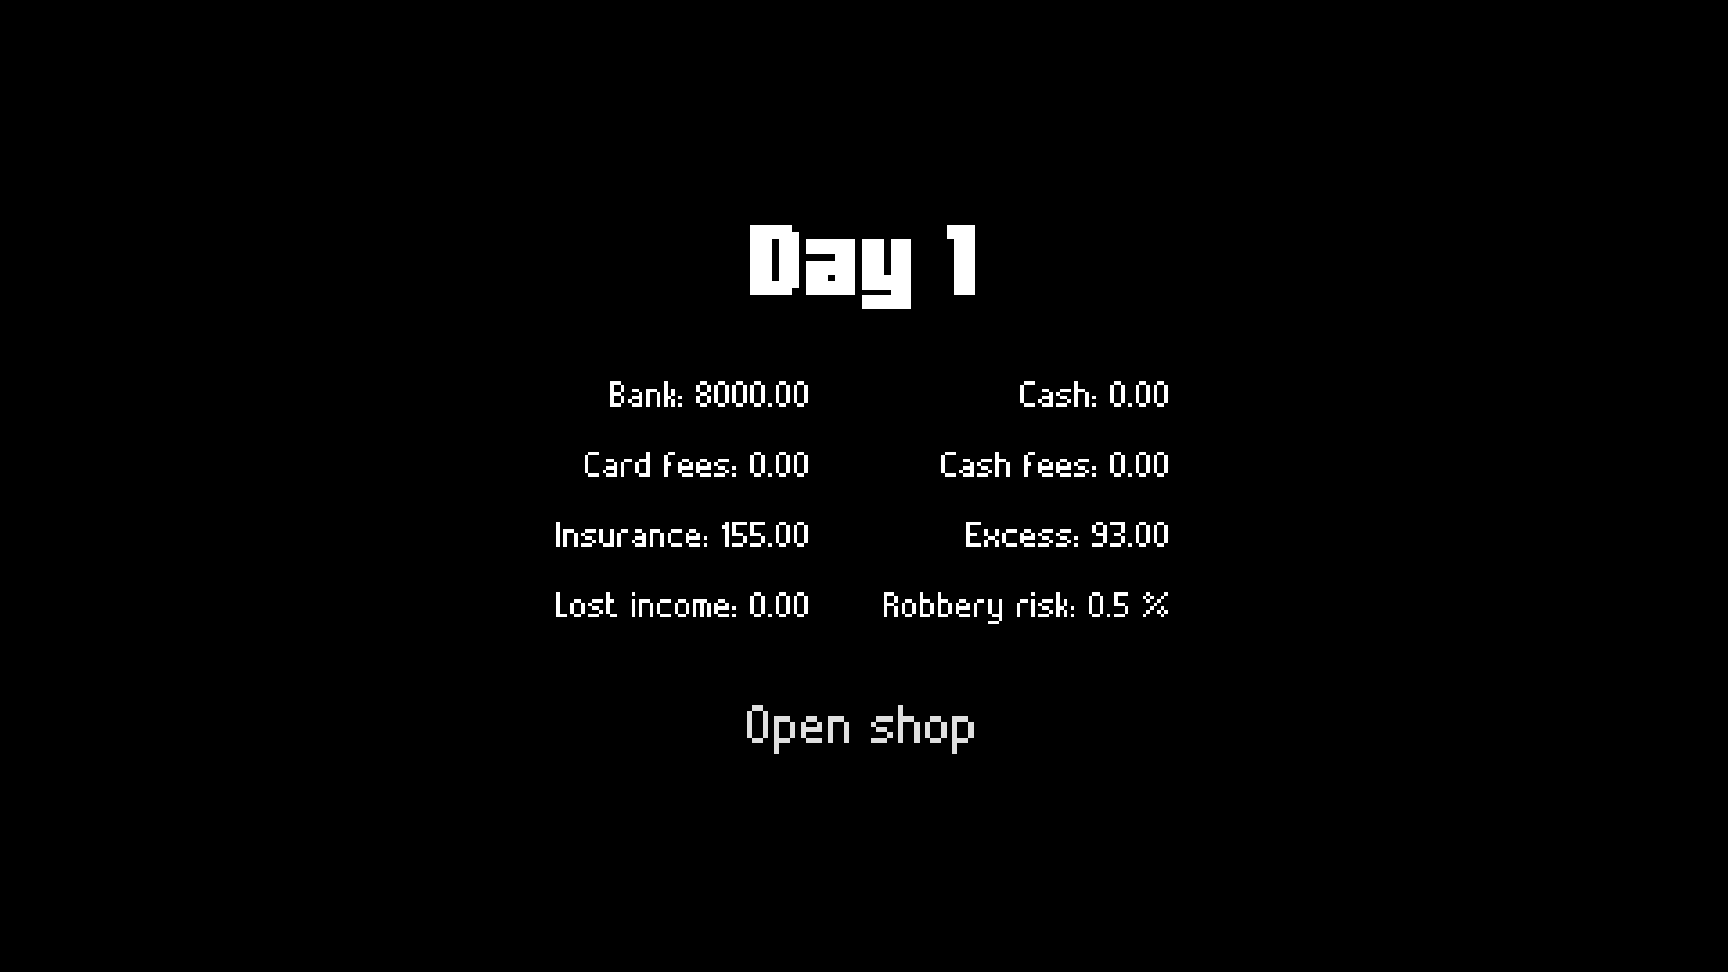
\includegraphics[width=\textwidth]{figures/day-card.png}
    \caption{Day card with the current state of play}\label{fig:day-card}
  \end{subfigure}
  \hfill
  \begin{subfigure}{0.475\textwidth}
    \centering
    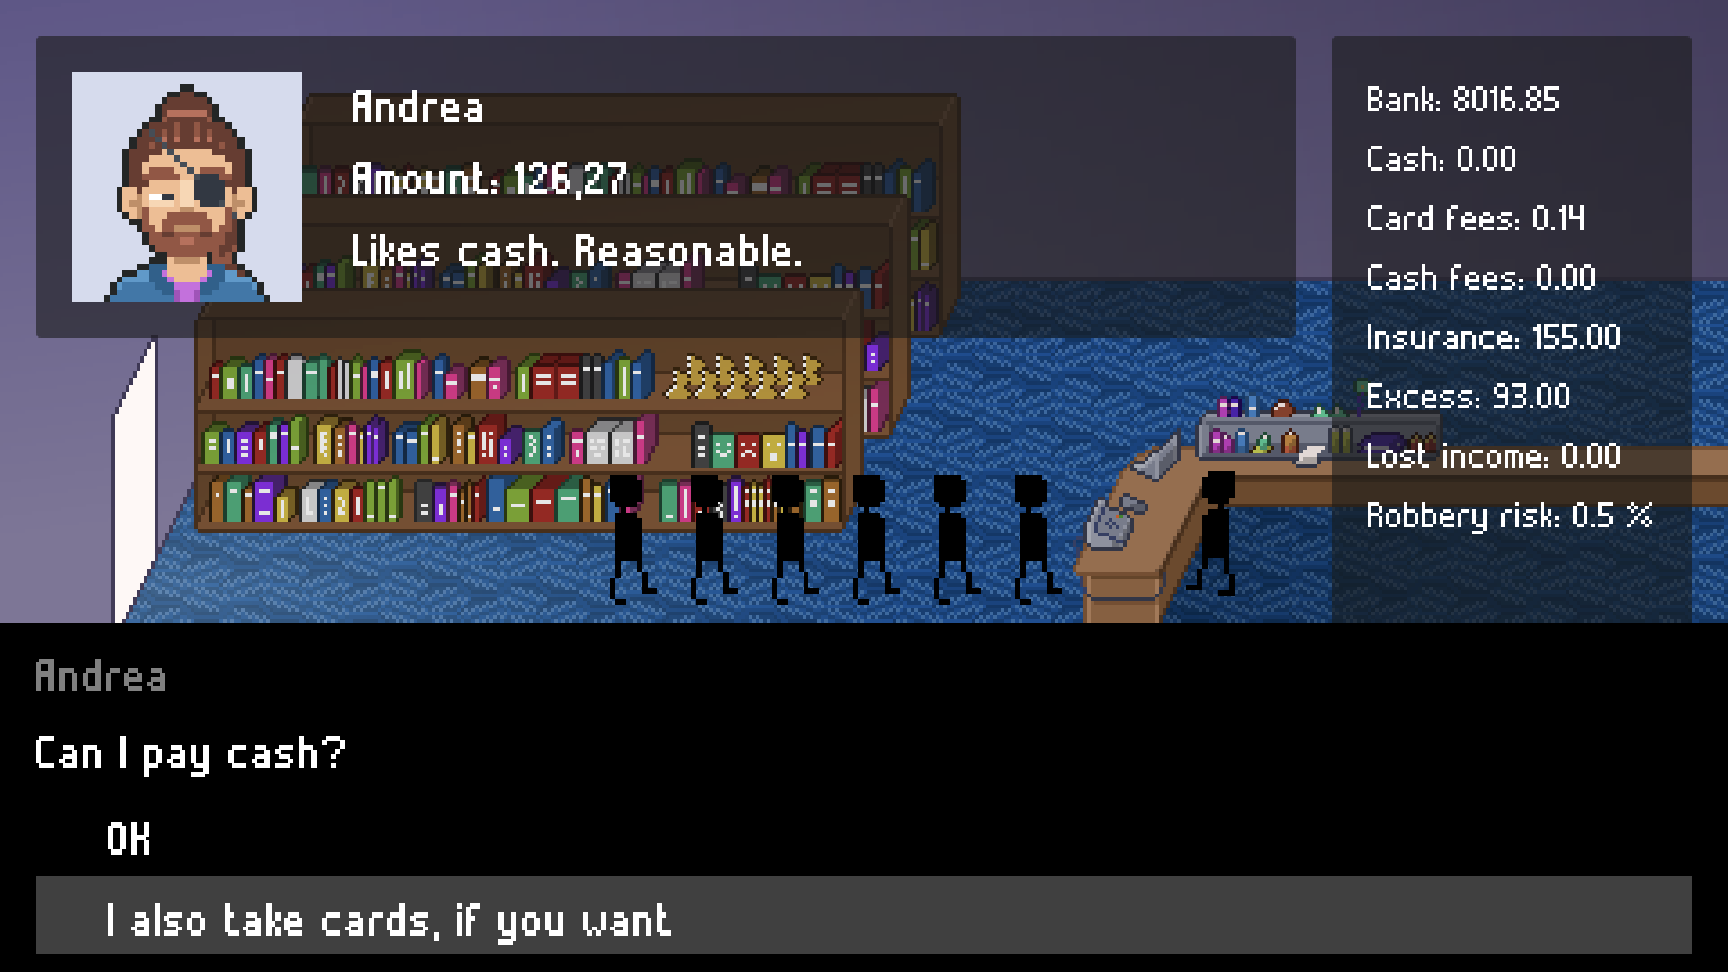
\includegraphics[width=\textwidth]{figures/gameplay.png}
    \caption{Main gameplay scene}\label{fig:gameplay}
  \end{subfigure}

  \vspace{\baselineskip}
  \begin{subfigure}{0.475\textwidth}
    \centering
    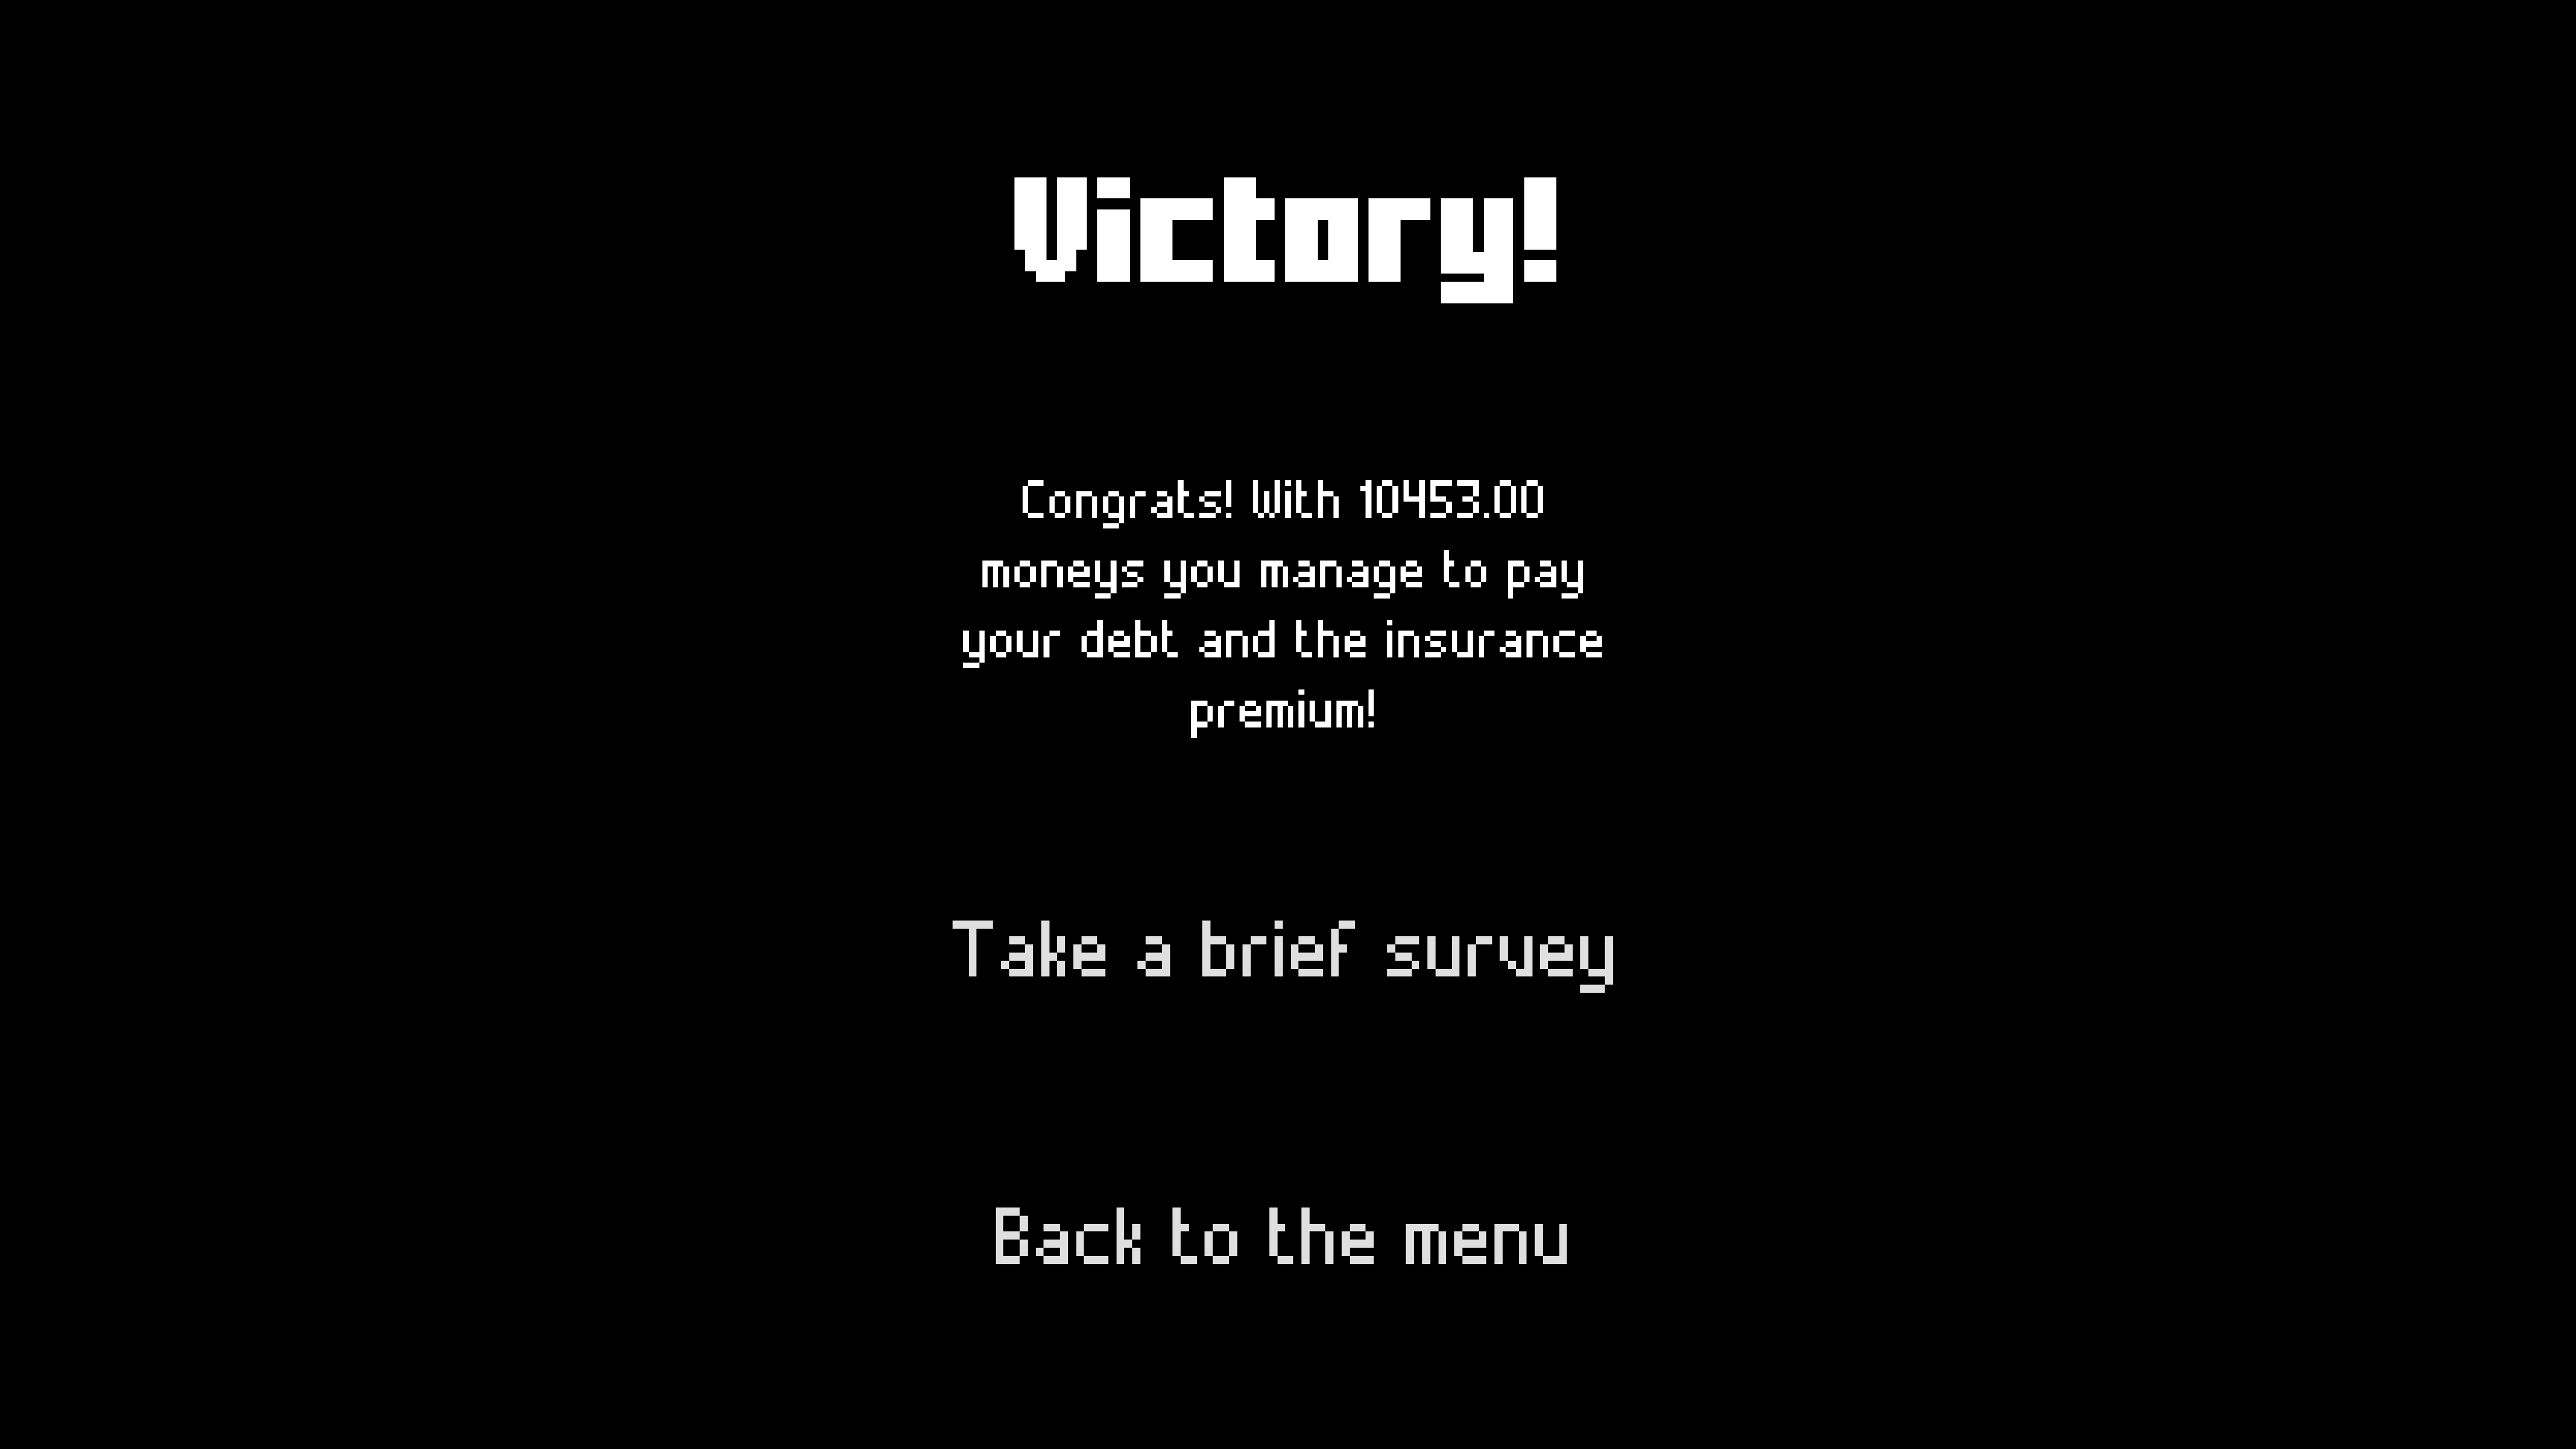
\includegraphics[width=\textwidth]{figures/victory.png}
    \caption{Victory screen}\label{fig:victory}
  \end{subfigure}
  \hfill
  \begin{subfigure}{0.475\textwidth}
    \centering
    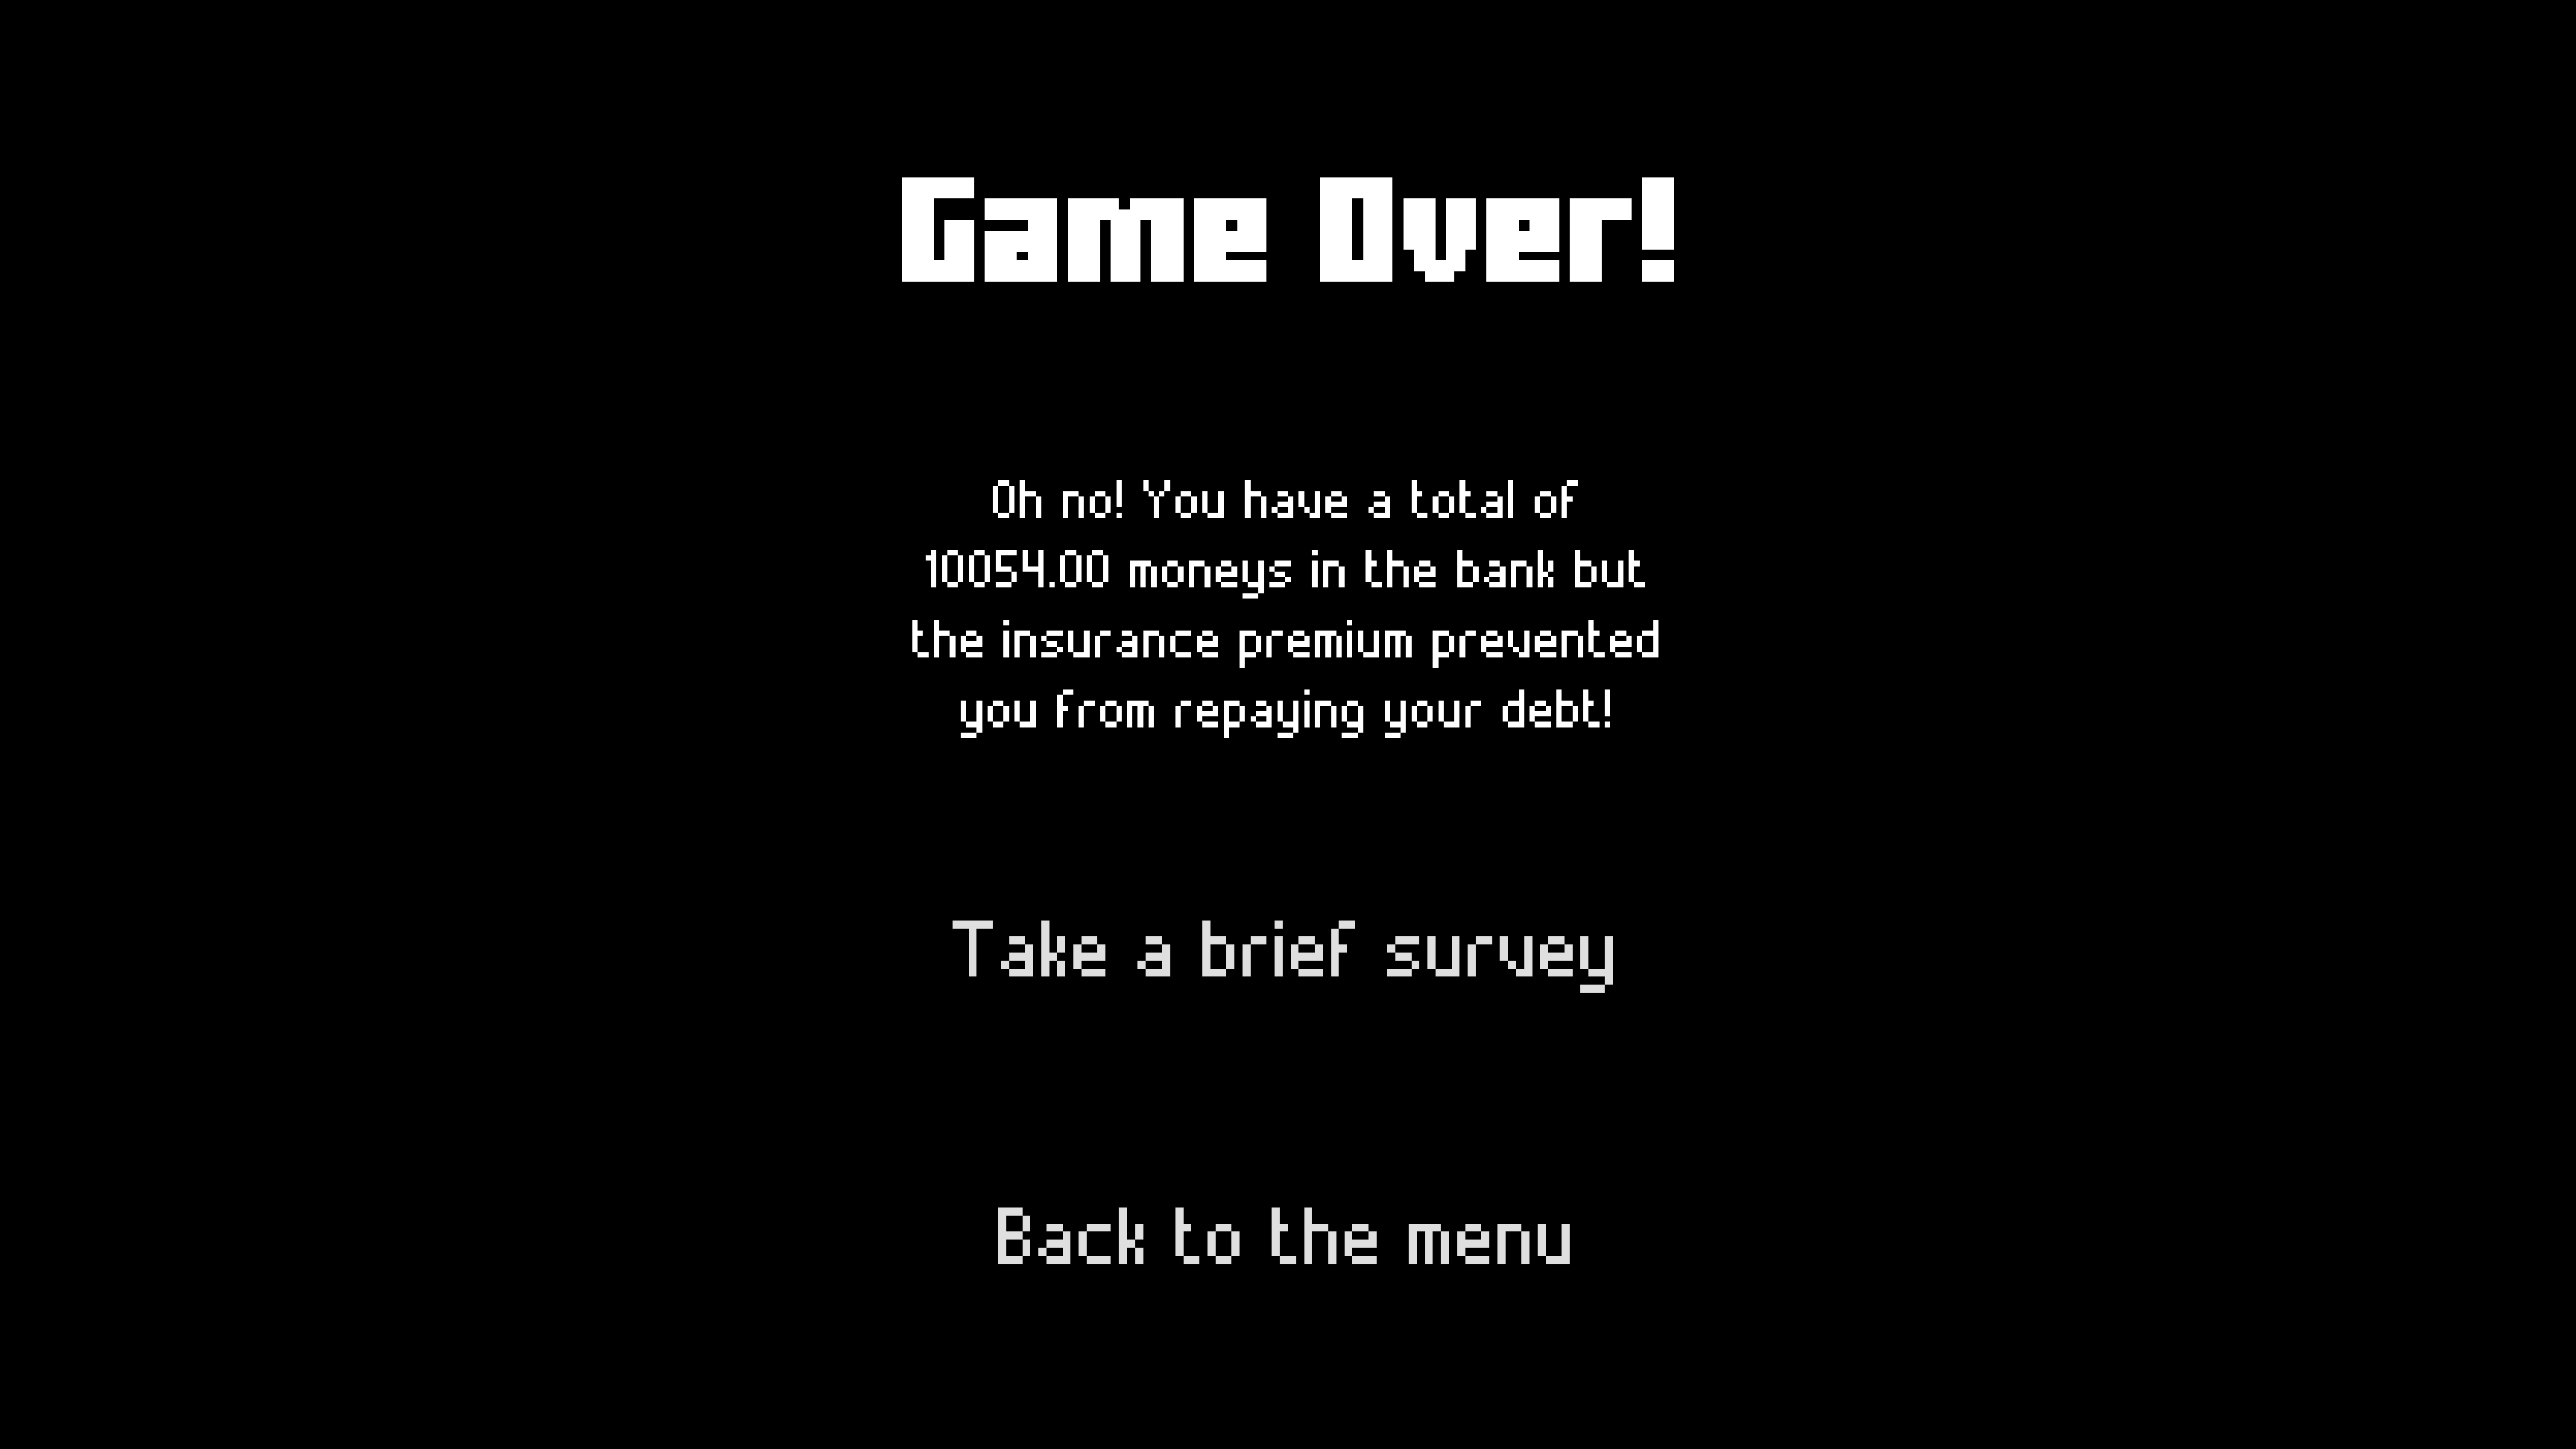
\includegraphics[width=\textwidth]{figures/game-over.png}
    \caption{Game over screen}\label{fig:game-over}
  \end{subfigure}

  \caption{}\label{fig:screens}
\end{figure}
  
\section{Strengths, Weaknesses, Opportunities, Threats}\label{swot}
The following analysis must be considered in the context of educational video games, as explained in \S\ref{background}.

\subsection{Strengths}
\begin{description}
  \item[Player freedom:] the game allows the player to choose their strategy, providing feedback in the form of objective metrics.
  \item[Player control:] the game has a clear win condition which is presented at the beginning, as part of the narrative which constitutes the main game fiction (\S\ref{game-world}).
  \item[Neutrality:] the game presents the issue of cash vs card payments in as neutral a way as possible.
  \item[Content presentation:] the content is woven into the gameplay and is central to the main game fiction.
\end{description}

\subsection{Weaknesses}
\begin{description}
  \item[Content presentation:] the content may feel a bit literal, it may be overly clear that the game is of the educational type and that it is trying to teach something, which some players may find unattractive.
  \item[Replayability:] once the player wins the game, which can happen during the first play-through, there is no particular incentive to play again.
\end{description}

\subsection{Opportunities}
\begin{description}
  \item[Power-ups:] there is scope for implementing additional elements that may change how the game plays out. Early ideas that have not yet been implemented include
  \begin{itemize}
    \item shop guard to reduce the risk of shop robbery;
    \item different positive and negative effects of different payment methods on running the shop;
    \item consequences of accepting or refusing more often a certain payment method.
  \end{itemize}
  \item[Expanded narrative:] e.g., include external events that impact the costs and opportunities of making certain choices.
  \item[Side mechanics:] e.g., re-negotiating the invoice payment, re-negotiating fees.
  \item[Trolling:] this can present an opportunity for increasing engagement in the game's theme and will be discussed among the threats in the next section.
\end{description}

\subsection{Threats}
\begin{description}
  \item[Existential:] the game is what is known as a ``news'' game, or a ``commentary'' game. These games are typically \textbf{only relevant for a limited amount of time}, often only while the issues discussed are relevant to society. It is hoped that the cash vs card debate will become less relevant in time, thus the relevance of this game will fade into historical interest at best. This is not necessarily a bad thing because it would imply that the game has served its purpose of educating and normalizing the co-existence of different payment methods, but it does pose a threat to the existence and relevance of the game nevertheless.
  \item[Trolling:] online trolling activity can affect the perception of the game. If played well, this can be turned into an opportunity to impact the public discourse about cash vs electronic payments. There is a very small chance that online trolling and animosity could migrate offline and produce real-life consequences for the individuals involved in making this game. The chance of this happening is negligible but not null.
\end{description}

\section{References}
\subsection{Gameplay}
The main inspiration for this game is ``Papers, Please'' by Lucas Pope, a puzzle simulation in which the player must make seemingly simple decisions based on a multitude of factors.

The main similarity between ``Cash or Card?'' and ``Papers, Please'' is that the player must interact with a line of people, one at a time, and make strategic decisions about each case, considering individual factors and the evolving state of the game.

\subsection{Visuals}
Retro-style pixel art is a popular art style for low-budget and independent video games. While it is possible to create highly sophisticated visuals in this style, it is also possible to get away with relatively reduced effort, provided that the work is sufficiently legible.

Player's focus on the gameplay is highly desirable in this kind of games, and pixel art has the advantage of making it easy to keep the visuals simple in order to avoid unnecessary distractions.

\subsection{Music}
Chiptune-style music fits well with the retro style of the game. The background music during gameplay is generic yet arousing in order to keep the player active while limiting distractions.

\end{document}
